
\subsection{Data qubit displacement}
The proposal \cite{OGorman2016} as described in section \ref{sec:PhysicalImplementation} utilises two distinct qubit arrays each of lattice constant $D$, separated by a distance $d$ perpendicular to the planes. To achieve reasonable interaction times compared to qubit decoherence times, distances $D = \SI{400}{\nano\metre}$ and $d = \SI{40}{\nano\metre}$ have been chosen for simulation.

It is may prove unrealistic, however, to expect to be able to deterministically place qubits with \si{\nano\metre} precision in a scalable manner. Resolutions of \SI{10}{\nano\metre} can be achieved using e-beam lithography \cite{Vieu2000a} or nanostencil masks \cite{Weis2008}, combined with single-ion implantation techniques \cite{Jamieson2005}. STM patterning techniques offer atomic precision of dopants in Si \cite{Schofield2003} but a method of maintaining this precision over an array several \si{\micro\metre} across remains elusive. 

To consider in detail the effect of these displacements, we generated uniformly random offsets to the position of each data qubit within a pillbox of heigh and radius $R$, as illustrated in fig.\@ \ref{fig:pillbox}. This form of displacement is the same as used in the proposal \cite{OGorman2016} and was chosen as the displacement in the $x$--$y$ plane would be expected to be uniformly radial, and the implantation depth in the $z$-axis would be independent from this.

To illustrate the errors qubit displacement creates, consider a set of typical qubit displacements as illustrated in fig.\@ \ref{fig:qubitdisplacements}. These displacements give each data qubit a different distance $r$ at which it is closest to the probe qubit as it passes overhead, resulting in a different interaction strength. Hence the phase accumulated for each data qubit varies from the ideal $\tfrac{\pi}{2}$ by an independent amount. These errors are systematic in that the same phases are picked up for each parity measurement, unlike the probe jitter considered in section \ref{sec:jitter}.

We find that for these displacements, the case of even parity (no bit-flips) yields close to a $2\pi$ evolution with $99.968\%$ probability of successfully measuring $\ket{+}$, from the evolution shown in fig.\@ \ref{fig:displacementnoerrors}. However, on introducing bit-flip errors to each of the four data qubits, different phase accumulations are observed as in fig.\@ \ref{fig:displacementerrors}.



[FIND A GOOD SPOT TO INSERT THIS LATER] This was considered in the proposal \cite{OGorman2016}, and using a simulation of the logical surface code operations a threshold of \SI{6.1}{\nano\metre} was derived.

[BELOW LIES OLD CRAP]\\
\\ 

The effect of displacement of the data qubits from the ideal was investigated. Ideally the data qubits would be in a square lattice of spins precisely $D = \SI{400}{\nano\metre}$ apart, but due to inaccuracies in dopant spin placement each qubit will have small displacements from the ideal lattice position.

This is modelled by generating a uniform random displacement within a given pillbox $xy$-radius and $z$-height. Simulations from the original paper show $\textrm{radius} = \textrm{height} = \SI{6}{\nano\metre}$ to be a threshold for this scheme. The phase accumulated over 25 runs for this pillbox size is plotted as a histogram in fig.\@ \ref{fig:DisplacementPhaseHistogram}, showing a maximum phase error of $\tfrac{\pi}{4}$ for these runs. 



The effect of displacements in the $x$-$y$ plane and the $z$-axis are significantly different in magnitudes, due to the $\tfrac{1}{d^3}$ term in the Hamiltonian being most strongly affected by $z$ displacements. This effect was investigated by artificially setting displacements in these directions.

Fig.\@ \ref{fig:zoffset} shows changes in accumulated phase due to $z$-displacements. The first 2 qubits are displaced \SI{4}{\nano\metre} down, slowing the evolution and giving a noticeable phase error after half a cycle. However, qubit 4 is displaced \SI{3}{\nano\metre} upwards, reducing $d$ and resulting in faster evolution. The effect is a small phase error from the ideal $2\pi$.

Fig.\@ \ref{fig:inwarddisplacement} shows the effect of displacements in the $x$-$y$ plane. For this run, all data qubits were displaced \SI{10}{\nano\metre} inwards with respect to the circular motion. The phase error on each individual qubit is then less than that produced by the \SI{3}{\nano\metre} $z$-displacement of fig.\@ \ref{fig:zoffset}, showing the smaller sensitivity to displacement in the $x$-$y$ plane, though the overall error after all 4 qubits is greater as in the $z$-direction, +$z$ and --$z$ errors cancel out somewhat, whereas $xy$ displacement errors will always slow the evolution.


\begin{figure*}
	\centering
%	\includegraphics[width=\columnwidth]{../Figures/pillbox.pdf}
	\subfloat[]{\includegraphics[width=0.7\columnwidth]{../figures/pillbox.pdf} \label{fig:pillbox}}
	\subfloat[]{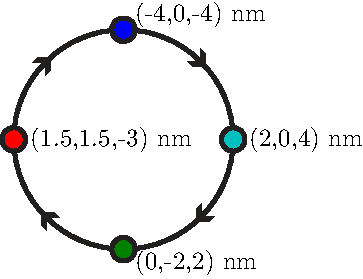
\includegraphics[width=0.7\columnwidth]{../figures/qubit_displacement_colours.pdf} \label{fig:qubitdisplacements}}
	\subfloat[]{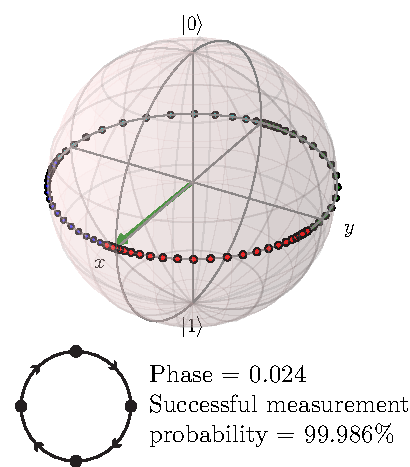
\includegraphics[width=0.5\columnwidth]{../figures/notwirl_noerror.pdf} \label{fig:displacementnoerrors}}
	
	\subfloat[]{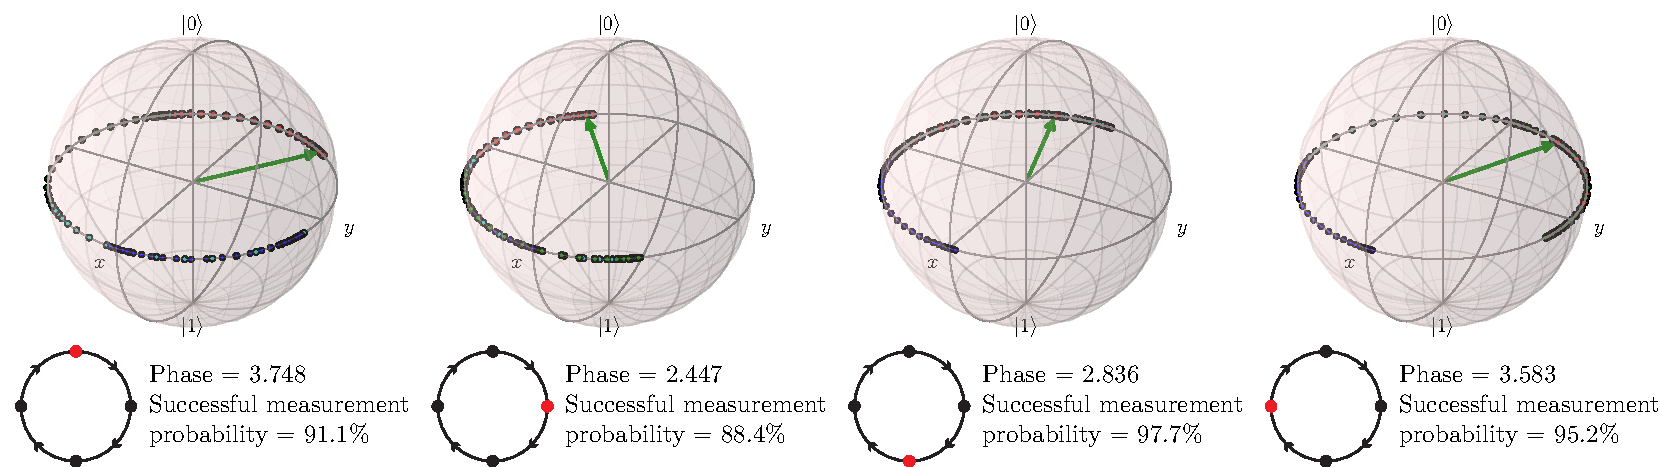
\includegraphics[width=2\columnwidth]{../figures/notwirl_allerrors_landscape.png} \label{fig:displacementerrors}}
	
	\caption{aoeu NOTE: change last subfigure to .pdf}
\end{figure*}

\begin{figure*}
	\centering
	\includegraphics[width=\textwidth]{../Figures/Displacement_Histogram.pdf}	
	\caption{Phase errors over 25 runs as a result of randomly generated data qubit displacements within a pillbox of half-height \SI{3}{\nano\metre} and radius \SI{6}{\nano\metre}. These values are a threshold for the proposed scheme.}
	\label{fig:DisplacementHistogram}
\end{figure*}



